\documentclass{beamer}
% imprimir
% \documentclass[handout]{beamer} 
% \usepackage{pgfpages}
% \pgfpagesuselayout{4 on 1}[a4paper,landscape,border shrink=5mm]

\mode<presentation> {
  \usetheme{Warsaw}
  \setbeamercovered{transparent}
}

\usebackgroundtemplate{
\includegraphics[width=\paperwidth]{format/libresoft-bg.png}}
\usepackage[spanish]{babel}
\usepackage[utf8]{inputenc}
\usepackage{graphics}
\usepackage{amssymb} % Simbolos matematicos

%\definecolor{libresoftgreen}{RGB}{162,190,43}
%\definecolor{libresoftblue}{RGB}{0,98,143}

%\setbeamercolor{titlelike}{bg=libresoftgreen}

%% Metadatos del PDF.
\hypersetup{  
  pdftitle={Security Overview},
  pdfauthor={Pedro Coca},
  pdfcreator={GSyC/Libresoft},
  pdfproducer=PDFLaTeX,
  pdfsubject={Systems Security},
}
%%

\begin{document}

\title{Security Management Introduction}
\subtitle{Arquitectura de servidores con software libre}
\institute{pcoca@libresoft.es} 
\author{Pedro Coca}
%\date{\today}
\date{1st April 2011}

\frame{
\maketitle
\begin{center}

\includegraphics[width=6cm]{format/gsyc-urjc}
\end{center}
}

\frame{
~
\vspace{4cm}

\begin{flushright}
{\small
(cc) 2011 Pedro Coca. \\
  This presentation is publised under the Creative Commons 3.0 Attribution, available at 
  \url{http://creativecommons.org/licenses/by/3.0/}
 

\bigskip

}
\end{flushright}
}
%%

\section{Introduction to Security Management}

\begin{frame}
\frametitle{Security Management: Introduction}
\begin{itemize}
\item Primary Concepts: C-I-A 
\item Confidentiality: Information Classification
\item Integrity: Data cannnot be altered without being detected
\item Availability: Fault tolerance, Single poing of failure, backups, etc.
\end{itemize}
\end{frame}

%%%%%%%%%%%%%%%%%%%%%%%%%%%%%%%%%%%%%%%%%%%%%%%%%%%%%%%%%%%%

\begin{frame}
\frametitle{Security Management: Introduction}
\begin{itemize}
\item Security is a comprehensive area, including:
  \begin{itemize}
  \item Risk Management
  \item Information Security Policies
  \item Guidelines, Baselines, Procedures and Standards
  \item Security organisation and education, etc
  \end{itemize}
\item The aim of security is to protect the company/entity and its assets
\end{itemize}
\end{frame}

%%%%%%%%%%%%%%%%%%%%%%%%%%%%%%%%%%%%%%%%%%%%%%%%%%%%%%%%%%%%


\begin{frame}
\frametitle{Security Management: Concepts}
\begin{itemize}
\item {\bf Identification}: means by which users identify themselves to the system
\item {\bf Authentication}: testing or reconciliation of evindence of users identity
\item {\bf Accountability}: system ability to determine actions of users within the system and identify the user
\item {\bf Authorisation}: rights and permissions granted to a user or process
\item {\bf Privacy}: Level of confidentiality and privacy protection of a user
\end{itemize}
\end{frame}


%%%%%%%%%%%%%%%%%%%%%%%%%%%%%%%%%%%%%%%%%%%%%%%%%%%%%%%%%%%%


\begin{frame}
\frametitle{Before talking more about security...}

\begin{itemize}
\item Libre software and Security
\item More or Less secure?
\end{itemize}

\end{frame}


%%%%%%%%%%%%%%%%%%%%%%%%%%%%%%%%%%%%%%%%%%%%%%%%%%%%%%%%%%%%

\begin{frame}
\frametitle{Security in Libre Software: Myths and facts}
\begin{itemize}

  \item Is Open Source Good for Security?
  \url{http://www.dwheeler.com/secure-programs/Secure-Programs-HOWTO/open-source-security.html}
  \item Risky business: Keeping security a secret
  \url{http://www.zdnet.com/news/risky-business-keeping-security-a-secret/127072}

\end{itemize}
\end{frame}

%%%%%%%%%%%%%%%%%%%%%%%%%%%%%%%%%%%%%%%%%%%%%%%%%%%%%%%%%%%%

\section{Coverity Scan}

\begin{frame}
\frametitle{FLOSS Security: facts}
\begin{itemize}
\item Coverity Scan Initiative
\item Launched on March 6, 2006 
\item In the first year of operation, over 6,000 software defects were fixed
\item FLOSS developers use the analysis results from the Coverity Scan service
\item In the first year, 50 open source projects written in C and C++ were included.
\end{itemize}
\end{frame}
%%%%%%%%%%%%%%%%%%%%%%%%%%%%%%%%%%%%%%%%%%%%%%%%%%%%%%%%%%%%

\begin{frame}
\frametitle{Coverity Scan}
\begin{itemize}
\item Coverity unveiled the expansion of Scan in the 1st year aniversary 
\item More projects were added
\item More information was made available for developers 
\item A new framework was put into place to help open source developers
\end{itemize}
\end{frame}

%%%%%%%%%%%%%%%%%%%%%%%%%%%%%%%%%%%%%%%%%%%%%%%%%%%%%%%%%%%%

\begin{frame}
\frametitle{Coverity Scan 2010}
\begin{itemize}
\item Coverity Scan 2010 experiment another transformation
\item Up to 291 projects
\item 191 out of 291 with active developer support
\item Over 61 million unique lines of code were tested
\item 49.654 defects identified 
\item ... and the open source community has fixed 15.278 of them.
\end{itemize}
\end{frame}


%%%%%%%%%%%%%%%%%%%%%%%%%%%%%%%%%%%%%%%%%%%%%%%%%%%%%%%%%%%%

\begin{frame}
\frametitle{Coverity Scan 2010. Defects}
\begin{center}
  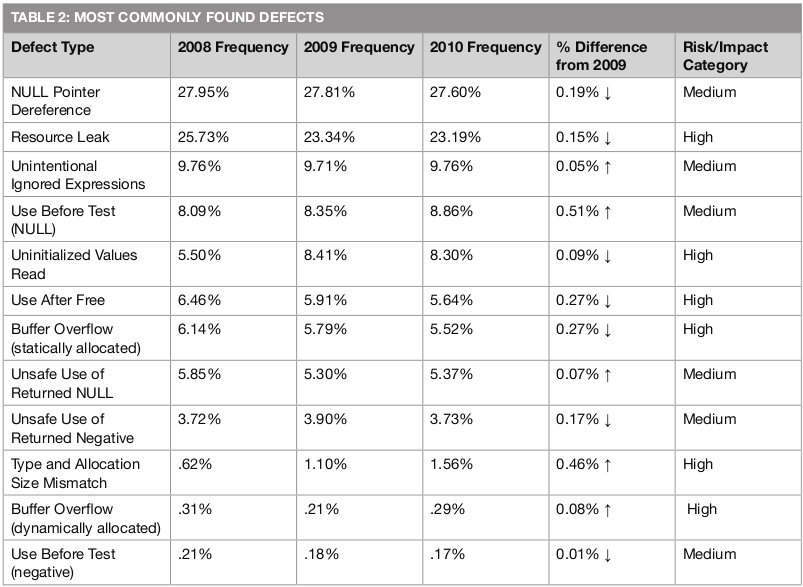
\includegraphics[width=9cm]{figs/Coverity_2010_Defects.png}
\end{center}
\end{frame}

%%%%%%%%%%%%%%%%%%%%%%%%%%%%%%%%%%%%%%%%%%%%%%%%%%%%%%%%%%%%

\begin{frame}
\frametitle{Coverity Scan. Integrity Levels }
\begin{itemize}
\item Coverity Integrity Level 1
    \begin{itemize}
    \item Defect density equals or less than 1 defect/kloc
    \end{itemize}
\item Coverity Integrity Level 2
    \begin{itemize}
    \item Defect density equals or less than 0.1 defect/kloc
    \item 90th industry percentile
    \end{itemize}
\item Coverity Integrity Level 3
    \begin{itemize}
    \item Defect density equals or less than 0.01 defect/kloc (99th industry percentile)
    \item Less than 20\% of the results
    \item Zero high defects
    \end{itemize}
\item Level Not Achieved
    \begin{itemize}
    \item Too many unresolved defects
    \end{itemize}
\end{itemize}
\end{frame}

%%%%%%%%%%%%%%%%%%%%%%%%%%%%%%%%%%%%%%%%%%%%%%%%%%%%%%%%%%%%


\begin{frame}
\frametitle{Coverity Scan 2010}
\begin{itemize}
\item Several popular projects (Firefox, Linux and PHP) were included before
\item Android kernel 2.6.32 (Froyo) was included in 2010
\begin{itemize}
\item Lines of Code Inspected: 765,642
\item Project Defect Density: 0.47 (defects per thousand lines of code)
\item High and Medium Impact Defects: 359
\end{itemize}
\end{itemize}
\end{frame}

%%%%%%%%%%%%%%%%%%%%%%%%%%%%%%%%%%%%%%%%%%%%%%%%%%%%%%%%%%%%

\begin{frame}
\frametitle{Coverity Scan 2010: Android Froyo}
\begin{center}
  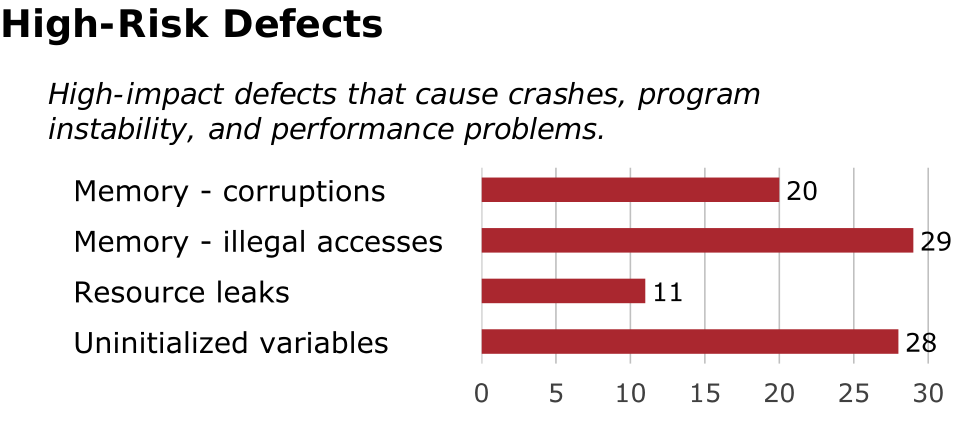
\includegraphics[width=11.3cm]{figs/Coverity_Froyo_High_Risk_Defects.png}
\end{center}
\end{frame}

%%%%%%%%%%%%%%%%%%%%%%%%%%%%%%%%%%%%%%%%%%%%%%%%%%%%%%%%%%%%

\begin{frame}
\frametitle{Coverity Scan 2010: Android Froyo}
\begin{center}
  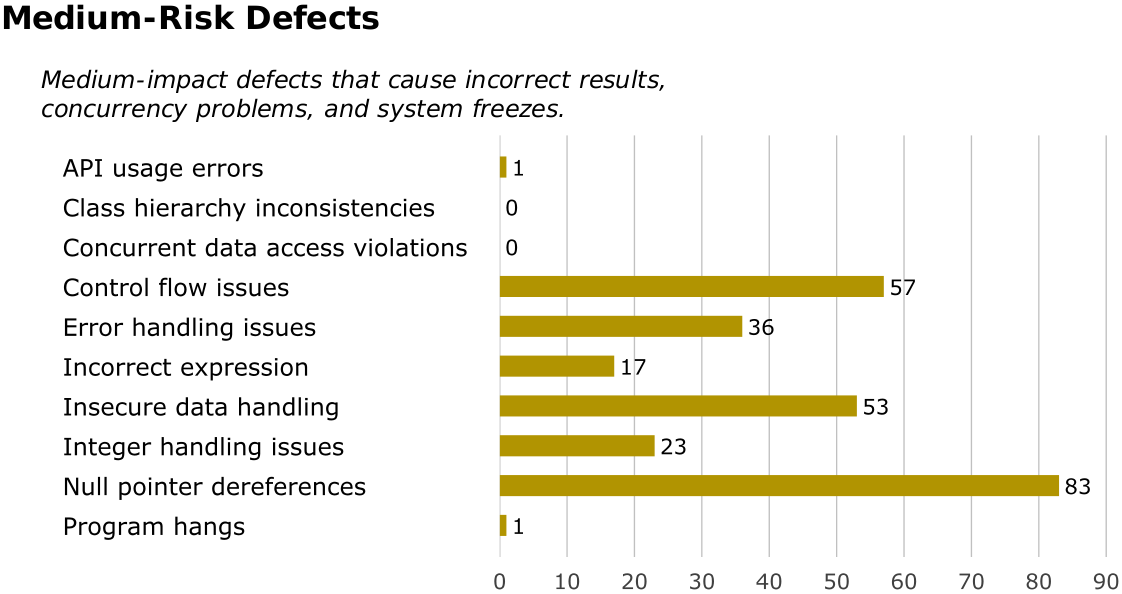
\includegraphics[width=11.3cm]{figs/Coverity_Froyo_Medium_Risk_Defects.png}
\end{center}
\end{frame}

%%%%%%%%%%%%%%%%%%%%%%%%%%%%%%%%%%%%%%%%%%%%%%%%%%%%%%%%%%%%

\begin{frame}
\frametitle{Coverity Scan 2010: Android Froyo}
\begin{itemize}
\item The Android kernel used in the HTC Droid Incredible has approximately half the defects that would be expected for average software of the same size.
\item Android-specific code that differs from the Linux kernel had about twice the defect density of the core Linux kernel components.
\end{itemize}
\end{frame}


%%%%%%%%%%%%%%%%%%%%%%%%%%%%%%%%%%%%%%%%%%%%%%%%%%%%%%%%%%%%

\begin{frame}
\frametitle{Coverity Scan}
\begin{itemize}
\item For more information and details, check out the 2008, 2009 and 2010 reports.
\end{itemize}
\begin{center}
\huge{Questions? / Comments?}
\end{center}
\end{frame}


%%%%%%%%%%%%%%%%%%%%%%%%%%%%%%%%%%%%%%%%%%%%%%%%%%%%%%%%%%%%

\section{Introduction to Risk Management}

\begin{frame}
\frametitle{Risk Management: Introduction}
\begin{itemize}
\item The aim of security is to protect the company/entity and its assets
\item Risk management
  \begin{itemize}
  \item Identifies these assets
  \item Point to the threats putting them in peril
  \item Estimates the potential loss and harm if the threat becomes reality
  \item Identify action plans to mitigate those risks
  \item Provide an economic balance between the safeguard implemented and the impact of the threat
  \end{itemize}
\end{itemize}
\end{frame}


\begin{frame}
\frametitle{Security Management: Definitions}
\begin{itemize}

\item Vulnerability
  \begin{itemize}
  \item Absence or weakness of a safeguard
  \item Is a HW or SW weakness that may provide an attacker a way to compromise our (CIA) system.
  \item Could be an open port, unpatched applications, unrestriced modem dial-in access, no physical security, etc,
  \end{itemize}
\item Threat
  \begin{itemize}
  \item Any event that causes an undesirable impact on our organisation.
  \item Any potential danger to the system or to the information.
  \item Could be a Tsunami, an unintentional mistake leading to confidential data exposure, a process reading data violating our data policy, etc
  \end{itemize}
\end{itemize}
\end{frame}


%%%%%%%%%%%%%%%%%%%%%%%%%%%%%%%%%%%%%%%%%%%%%%%%%%%%%%%%%%%%

\begin{frame}
\frametitle{Security Management: Definitions}
\begin{itemize}

\item Risk
  \begin{itemize}
  \item Is the probability of a threat agent exploiting a vulnerability and the corresponding business impact
  \item Potential lost or harm to a system.
  \item If there is no IDS, the risk (likelihood) of unnoticed attacks would be high
  \item If there is no awareness training, the risk of unintentional mistakes causing information deletion/exposure would be high
  \end{itemize}
\item Exposure
  \begin{itemize}
  \item Is an instance of being exposed to harm or lost from an entity that takes advantage of a vulnerability
  \end{itemize}
\end{itemize}
\end{frame}

%%%%%%%%%%%%%%%%%%%%%%%%%%%%%%%%%%%%%%%%%%%%%%%%%%%%%%%%%%%%

\begin{frame}
\frametitle{Security Management: Definitions}
\begin{itemize}

\item Safeguard
  \begin{itemize}
  \item Is the countermeasure to put in place to mitigate the potential risk
  \item Could be a procedure, a piece of HW or SW, etc
  \item Access Controls, strong password management policies, awareness training, etc
  \end{itemize}
\end{itemize}
\end{frame}

%%%%%%%%%%%%%%%%%%%%%%%%%%%%%%%%%%%%%%%%%%%%%%%%%%%%%%%%%%%%

\begin{frame}
\frametitle{Security Management: Risk Management}
\begin{itemize}

\item Information Risk Management (IRM)
  \begin{itemize}
  \item The prime objective of security controls is to reduce effects of theats and vulnerabilities to a level that is tolerable
  \item We have to implement the right mechanism to set and keep that level of risk
  \end{itemize}
\item Types of Risk
  \begin{itemize}
  \item There are many risk categories: Physical damage, Human interaction, Equipment malfunction, Inside and ouside attacks, Misuse of data, Loss of data and Application errors.
  \end{itemize}
\end{itemize}
\end{frame}

%%%%%%%%%%%%%%%%%%%%%%%%%%%%%%%%%%%%%%%%%%%%%%%%%%%%%%%%%%%%%%

\begin{frame}
\frametitle{Security Management: Risk Analysis}
\begin{itemize}

\item Risk Analysis Objectives
  \begin{itemize}
  \item Identify assets and their values
  \item Identify vulnerabilities and threats 
  \item Quantifying the probability and business impact of these potential threats
  \item Provide an economic balance between the impact of the threat and the cost of the countermeasure 
  \end{itemize}
\end{itemize}
\end{frame}

%%%%%%%%%%%%%%%%%%%%%%%%%%%%%%%%%%%%%%%%%%%%%%%%%%%%%%%%%%%%%%

\begin{frame}
\frametitle{Security Management: Risk Analysis}
\begin{itemize}
\item Risk Analysis can take two approaches:
\item {\bf Quantitative} Risk Analysis 
\item {\bf Qualitative} Risk Analysis 
\item Each approach has advantages and disadvantages
\end{itemize}
\end{frame}


%%%%%%%%%%%%%%%%%%%%%%%%%%%%%%%%%%%%%%%%%%%%%%%%%%%%%%%%%%%%%%

\begin{frame}
\frametitle{Security Management: Risk Analysis}
\begin{itemize}

\item Risk Analysis Steps
  \begin{itemize}
  \item Assign Value to Assets
  \item Estimate potential loss per threat
  \item Carry out a threat analysis
  \item Derive the Overall Loss Potential per Threat
  \item Reduce, Transfer or Accept the risk
  \end{itemize}
\end{itemize}
\end{frame}


%%%%%%%%%%%%%%%%%%%%%%%%%%%%%%%%%%%%%%%%%%%%%%%%%%%%%%%%%%%%%%


\begin{frame}
\frametitle{Security Management: Risk Analysis}
\begin{itemize}

\item Value of Assets
  \begin{itemize}
  \item Quantitative and Qualitative measures 
  \item The actual value of an asset is determined by the cost to acquire, develop and maintain it.
  \item Value of the asset to owners and users
  \item Value of the asset to competitors
  \item Intelectual property issues
  \item Liability issues (Data protection)
  \item It is critical to take into account the business impact!
  \end{itemize}
\end{itemize}
\end{frame}

%%%%%%%%%%%%%%%%%%%%%%%%%%%%%%%%%%%%%%%%%%%%%%%%%%%%%%%%%%%%%%


\begin{frame}
\frametitle{Security Management: Risk Analysis}
\begin{itemize}

\item Identifying Threats
  \begin{itemize}
  \item Viruses, Attackes, Intruders
  \item Physical Threats
  \item Employees / Users / Contractors
  \item Gather information about the probability of each threat
  \item Calculate the annualised rate of occurrence (ARO)
  \end{itemize}
\end{itemize}
\end{frame}


%%%%%%%%%%%%%%%%%%%%%%%%%%%%%%%%%%%%%%%%%%%%%%%%%%%%%%%%%%%%%%

\begin{frame}
\frametitle{Security Management: Risk Analysis}
\begin{itemize}

\item Reduce, Transfer or Accept the Risk
  \begin{itemize}
  \item Reducing the risk:
     \begin{itemize}
     \item Set controls
     \item Improve procedures
     \item Security awareness training
     \item ...
     \end{itemize}
  \item Transfering the risk:
     \begin{itemize}
     \item Insurance
     \end{itemize}
  \item Accepting the riks:
     \begin{itemize}
     \item Stop using resources for protection and live with the risk
     \end{itemize}
  \end{itemize}
\end{itemize}
\end{frame}


%%%%%%%%%%%%%%%%%%%%%%%%%%%%%%%%%%%%%%%%%%%%%%%%%%%%%%%%%%%%%%


\begin{frame}
\frametitle{Security Management: Risk Analysis}
\begin{itemize}

\item Risk Analysis Results
  \begin{itemize}
  \item Monetary values assigned to assets
  \item Comprehensive list of all possible and significant threats
  \item Likelyhood of the occurence rate (for each threat)
  \item Potential loss that the company/entity can endure per threat in a timely basis
  \item Recommended safeguards, remediation actions, countermeasures
  \end{itemize}
\item Residual Risk

\end{itemize}

\end{frame}


%%%%%%%%%%%%%%%%%%%%%%%%%%%%%%%%%%%%%%%%%%%%%%%%%%%%%%%%%%%%
\section{Introduction to Access Control}
%%%%%%%%%%%%%%%%%%%%%%%%%%%%%%%%%%%%%%%%%%%%%%%%%%%%%%%%%%%%
\begin{frame}
\frametitle{Access Control Definition}

\begin{itemize}
\item Set of procedures perfomed by hardware, software and administrative items
\item Aimed to:
   \begin{itemize}
   \item Monitor access
   \item Identify user requesting access
   \item Record access attepmpts
   \item Grant or deny access based on a pre-established rules
   \end{itemize}
\end{itemize}

\end{frame}

%%%%%%%%%%%%%%%%%%%%%%%%%%%%%%%%%%%%%%%%%%%%%%%%%%%%%%%%%%%%
\begin{frame}
\frametitle{Access Control Principles}

\begin{itemize}
\item As we have just seen, the three main principles for any type of control are:
\begin{itemize}
\item Confidentiality
\item Integrity
\item Availability
\end{itemize}
\end{itemize}

\end{frame}


%%%%%%%%%%%%%%%%%%%%%%%%%%%%%%%%%%%%%%%%%%%%%%%%%%%%%%%%%%%%
\begin{frame}
\frametitle{Access Control Models: MAC}

\begin{itemize}
\item Mandatory Access Control
    \begin{itemize}
    \item Subjects have a {\bf clearance}
    \item Objects have a {\bf classification}
    \item Subjects must have a {\bf need to know} over the Objects
    \item Subjects can access Objects with the same or below clearance level and a need to know for the Objects
    \item Rule-based access control is a type of MAC (access is not based on identity)
    \item Unclassified, confidential, secret and top secret {\bf sensitivity}
    \item SELinux, TrustedBSD are examples of Free OS implementing MAC
    \end{itemize}
\end{itemize}

\end{frame}

%%%%%%%%%%%%%%%%%%%%%%%%%%%%%%%%%%%%%%%%%%%%%%%%%%%%%%%%%%%%

\begin{frame}
\frametitle{Access Control Models: DAC}

\begin{itemize}
\item Discretionary Access Control
    \begin{itemize}
    \item The subject can specify (with limitations) what objects are accessible
    \item Access Control Lists (ACL) can be set up
    \item ACL shows what subjects can use what objects with what privileges
    \item Common Unix system of users, groups, and read-write-execute permissions
    \item Identity-based access controls
    \end{itemize}
\end{itemize}
\end{frame}


%%%%%%%%%%%%%%%%%%%%%%%%%%%%%%%%%%%%%%%%%%%%%%%%%%%%%%%%%%%%

\begin{frame}
\frametitle{Access Control Models: Non DAC}

\begin{itemize}
 
\item Non-Discretionary Access Control
    \begin{itemize}
    \item Also known as Role-based access control (RBAC)
    \item Assigning a user to a role is imposed (Always)
    \item A central Authority determines access between subjects and objects
    \item Access controls can be role-based or task-based
    \item These kind of control do not need to be updated if there is a role change in the company
    \item is RBAC a type of MAC?
       \begin{itemize}
       \item \url{http://csrc.nist.gov/rbac}
       \end{itemize}
    \end{itemize}

\end{itemize}
\end{frame}



%%%%%%%%%%%%%%%%%%%%%%%%%%%%%%%%%%%%%%%%%%%%%%%%%%%%%%%%%%%%
\begin{frame}
\frametitle{Access Control Models Wrap up}

\begin{itemize}
\item {\bf MAC}: Operating Systems, using security labels, enforce the model and therefore ther securiy system
\item {\bf DAC}: Data owners decide which subjects has access to which objects
\item {\bf RBAC}: Access to objects is determined by the role of each subject
\end{itemize}

\end{frame}

%%%%%%%%%%%%%%%%%%%%%%%%%%%%%%%%%%%%%%%%%%%%%%%%%%%%%%%%%%%%

\begin{frame}
\frametitle{Access Control Types}

\begin{itemize}
\item Preventive (Inhibit)
\item Detective (Discover)
\item Corrective (Restoring)
\end{itemize}

\end{frame}

%%%%%%%%%%%%%%%%%%%%%%%%%%%%%%%%%%%%%%%%%%%%%%%%%%%%%%%%%%%%
\begin{frame}
\frametitle{Access Control Implementation}

\begin{itemize}
\item Access Controls can be implemented with a set of measures:
\begin{itemize}
\item {\bf Administrative}
    \begin{itemize}
    \item Policies, procedures, staff training, reviews.
    \end{itemize}
\item {\bf Logical/Technical}
    \begin{itemize}
    \item ACL, Firewalls, Smart Card Access, Encryption, etc
    \end{itemize}
\item {\bf Physical}
    \begin{itemize}
    \item Server Facilities locking, backing up, cable protection, etc
    \end{itemize}
\end{itemize}
\end{itemize}

\end{frame}

%%%%%%%%%%%%%%%%%%%%%%%%%%%%%%%%%%%%%%%%%%%%%%%%%%%%%%%%%%%%
\begin{frame}
\frametitle{Access Control Attacks}

\begin{itemize}

\item Denial of Service
  \begin{itemize}
  \item Compromises the availability
  \item Buffer Overflows, SYN Attack, etc
  \item Authorisation
  \end{itemize}
\item Back Door
  \begin{itemize}
  \item Bypasses access control mechanisms
  \end{itemize}
\item Spoofing, Man in the Middle, Session Hijacking, Social Engineering.
\item Dumpster diving
\item Password guessing, Brute Force, Dictionary Attacks
\item Software exploits, Trojan Horses, etc

\end{itemize}

\end{frame}



%%%%%%%%%%%%%%%%%%%%%%%%%%%%%%%%%%%%%%%%%%%%%%%%%%%%%%%%%%%%
\begin{frame}
\frametitle{Access Accountability}

\begin{itemize}
\item Access Controls provide Access Accountability 
\item Access Accountability needs:
  \begin{itemize}
  \item Identification
  \item Authentication
  \item Authorisation
  \end{itemize}
\end{itemize}

\end{frame}


%%%%%%%%%%%%%%%%%%%%%%%%%%%%%%%%%%%%%%%%%%%%%%%%%%%%%%%%%%%%
\begin{frame}
\frametitle{Identification, Authentication and Authorisation}

\begin{itemize}
\item {\bf Identification} sets a method of ensuring that a user, program or process (any subject) is the entity it claims to be.
  \begin{itemize}
  \item Usernames, Account numbers are ways to identify a subject
  \end{itemize}
\item {\bf Authentication} is the fact of confirming an identity claim made by or about the subject
  \begin{itemize}
  \item Passwords, PINs, Criptographic key, etc are usually authentication methods
  \end{itemize}
\item {\bf Authorisation} is the procedure of specifying access rights to a set of resources
  \begin{itemize}
  \item Usually the system checks an access control matrix or an ACL
  \end{itemize}
\end{itemize}

\end{frame}

%%%%%%%%%%%%%%%%%%%%%%%%%%%%%%%%%%%%%%%%%%%%%%%%%%%%%%%%%%%%
\begin{frame}
\frametitle{Strong Authentication}

\begin{itemize}

\item There are 3 general aspects to prove be authenticated:

\begin{itemize}
  \item Something you {\bf KNOW}
    \begin{itemize}
    \item Usually a PIN, password, etc
    \item Easy and cheap to implement
    \end{itemize}
  \item Something you {\bf HAVE}
    \begin{itemize}
    \item Usually a key, a badge, etc
    \item Normally used for physical access, but can be required for logical access
    \end{itemize}
  \item Something you {\bf ARE}
    \begin{itemize}
    \item Biometrics
    \item Complex and expensive implementation.
    \item False positives/negatives (Type I/II errors). Crossover rate
    \end{itemize}
\end{itemize}

\item {\bf Strong Authentication} contains 2 out of 3 aspects. Also know as {\bf two-factor authentication}

\end{itemize}

\end{frame}

%%%%%%%%%%%%%%%%%%%%%%%%%%%%%%%%%%%%%%%%%%%%%%%%%%%%%%%%%%%%
\begin{frame}

\frametitle{Passwords}

\begin{itemize}
\item Most common authentication method: User id bound with a reusable password.
\item Also weakest method!
\item Therefore, usually access control relies on password strength
\item Becomes very important the password management policy
\item Is an important target in attacks
\item Tools to analise the targeted social network profiles to create custom dicts
\item Tools to create non-dictionary tipical human variations
\end{itemize}

\end{frame}


%%%%%%%%%%%%%%%%%%%%%%%%%%%%%%%%%%%%%%%%%%%%%%%%%%%%%%%%%%%%
\begin{frame}

\frametitle{Password gathering techniques}

\begin{itemize}
\item Monitoring
\item Accessing the password file
\item Brute force attacks
\item Dictionary attacks
\item Social engineering
\end{itemize}

\end{frame}

%%%%%%%%%%%%%%%%%%%%%%%%%%%%%%%%%%%%%%%%%%%%%%%%%%%%%%%%%%%%
\begin{frame}

\frametitle{Password protection measures}

\begin{itemize}
\item Set a clipping Level (user will locked out for a fixed time)
\item Limit the number of failed logon attempts
\item Awareness training
\item Password checkers
\item Password hashing and Encryption
\item Password aging
\item Cognitive passwords
\item One-Time passwords  (dinamic passwords)
\item Token devices
   \begin{itemize}
   \item Synchronous
   \item Asynchronous (challenge/response)
   \end{itemize}
\end{itemize}

\end{frame}

%%%%%%%%%%%%%%%%%%%%%%%%%%%%%%%%%%%%%%%%%%%%%%%%%%%%%%%%%%%%

\section{Access Control Assignment}

%%%%%%%%%%%%%%%%%%%%%%%%%%%%%%%%%%%%%%%%%%%%%%%%%%%%%%%%%%%%

\begin{frame}

\frametitle{Access Control Assignment}
\begin{itemize}
\item Password strenght audit
\item Using a well known GPL password cracker: John the ripper
\item Add test users with increasing password complexity
\item Perform a password strengh audit in your own system
\item Measure the time needed to crack the password with the password complexity
\end{itemize}

\end{frame}

%%%%%%%%%%%%%%%%%%%%%%%%%%%%%%%%%%%%%%%%%%%%%%%%%%%%%%%%%%%%

\begin{frame}

\frametitle{Access Control Assignment}
\begin{itemize}
\item Download John the ripper software
\item Download "SHA-512" patch, so hashes can be loaded (Recent Ubuntu and Fedora)
\item Apply the patch and compile the patched john source code
\item Unshadow the password file 
\item Proceed to audit the file
\end{itemize}

\end{frame}

%%%%%%%%%%%%%%%%%%%%%%%%%%%%%%%%%%%%%%%%%%%%%%%%%%%%%%%%%%%%

\begin{frame}

\frametitle{Access Control Assignment}
\begin{itemize}
\item Of course, there are other good alternatives password audit FLOSS:
   \begin{itemize}
   \item {\bf THC Indra}
   \item \url{http://www.thc.org/thc-hydra/}
   \item {\bf Aircrack}
   \item \url{http://www.aircrack-ng.org/}
   \item {\bf Airsnort}
   \item \url{http://airsnort.shmoo.com/}
   \end{itemize}
\end{itemize}

\end{frame}

%%%%%%%%%%%%%%%%%%%%%%%%%%%%%%%%%%%%%%%%%%%%%%%%%%%%%%%%%%%%


\begin{frame}
\frametitle{John the ripper: GPL Password Audit Tool screenshot}
\begin{center}
  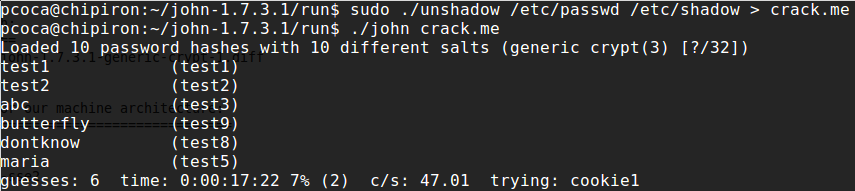
\includegraphics[width=11.3cm]{figs/John_ScreenShot.png}
\end{center}
\end{frame}


%%%%%%%%%%%%%%%%%%%%%%%%%%%%%%%%%%%%%%%%%%%%%%%%%%%%%%%%%%%%

\begin{frame}

\frametitle{Access Control Questions}
\begin{center}
\huge{How can the cheap and easy access to compute power in the cloud change the access control landscape?}
\end{center}
\end{frame}

%%%%%%%%%%%%%%%%%%%%%%%%%%%%%%%%%%%%%%%%%%%%%%%%%%%%%%%%%%%%

\begin{frame}
\frametitle{Access Control Questions}
\begin{itemize}

\item Cloud Cracking Suite presentation at Black Hat EU 2011:
   \begin{itemize}
   \item \url{https://stacksmashing.net/stuff/bh_eu_2011.pdf}
   \end{itemize}

\item Cracking Passwords In The Cloud: Amazon’s New EC2 GPU Instances 
   \begin{itemize}
   \item \url{http://stacksmashing.net/2010/11/15/cracking-in-the-cloud-amazons-new-ec2-gpu-instances/}
   \end{itemize}

\item Researcher uses AWS cloud to crack Wi-Fi passwords 
   \begin{itemize}
   \item \url{http://www.zdnet.co.uk/news/cloud/2011/01/14/researcher-uses-aws-cloud-to-crack-wi-fi-passwords-40091430}
   \end{itemize}

\end{itemize}

\end{frame}

%%%%%%%%%%%%%%%%%%%%%%%%%%%%%%%%%%%%%%%%%%%%%%%%%%%%%%%%%%%%

\begin{frame}
\frametitle{Questions?}
\begin{center}
\huge{Questions? / Comments?}
\end{center}
\end{frame}

%%%%%%%%%%%%%%%%%%%%%%%%%%%%%%%%%%%%%%%%%%%%%%%%%%%%%%%%%%%%
\end{document}
